%!TEX root = ../../../root.tex

As we have seen, defining convolution in the Fourier domain has an inherent drawback of inability to adapt the models across different domains. We will therefore need to resort to an alternative generalization of the convolution, now directly in the \emph{spatial} domain, i.e. the domain in which data naturally lives. However, even this second operation will not be a ``proper'' convolution.

Many recent works have proposed their approaches to defining convolution on general surfaces. However, basically all of them have to give up on translation invariance, and define some convolution-like operators that shares some other properties with convolution.

On a Euclidean domain, due to shift-invariance the convolution can be thought of as passing a template at each point of the domain and recording the correlation of the template with the function (e.g., an image) at that point (e.g., a pixel). Thinking of image filtering, this amounts to extracting a patch of pixels, multiplying it element-wise with a template (the filter) and summing up the results, then moving on to the next position in a sliding window manner. Shift-invariance implies that the very operation of extracting the patch at each position is always the same.

However, we have seen how on non-Euclidean domains we cannot even define correctly the notion of shift, let alone shift-invariance of operators. Therefore, extracting a local ``patch'' would be position-dependent. Furthermore, we have seen how it is difficult to globally parametrize a manifold, therefore it is not clear how to define \emph{adjacency} to even extract a \emph{local} patch. Given a certain point, what is local and what is not?

So, one of the properties that we want to recover is \emph{locality}. So, for each node $i$, we could define a local system of (polar) coordinates $\vb{u}_{ij}$ in which node $i$ is the origin, and every other point (node or point in the face) is identified in terms of radius and angle wrt an axis going from $i$ to some other point $j$. 
\begin{figure}[H]
	\centering
	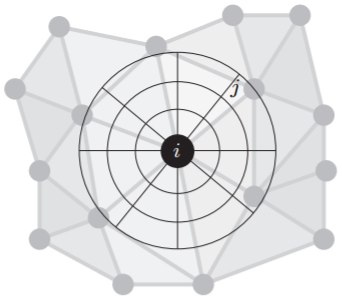
\includegraphics[width=.3\textwidth]{12/22_46_a}
	\caption{Local system of coordinates.}\label{fig:local-coord}	
\end{figure}

Now, how many nodes should we consider when extracting a \emph{local} patch? To enforce locality we should give more weight to closer nodes and less to further nodes. This is done with exponentially decaying local weights defined by means of several Gaussians, according to some quantization.

\begin{equation}
	w_{i, j} = exp\left( - \left( \mathbf{u}_{ij} - \mathbf{\mu} \right)^\top \mathbf{\Sigma}^{-1} \left( \mathbf{u}_{ij} - \mathbf{\mu} \right) \right)
\end{equation}
The mean and variances of these Gaussians are learnable, meaning that the model can learn that some nodes have more influence than others in the neighborhood of each node.

\begin{figure}[H]
	\centering
	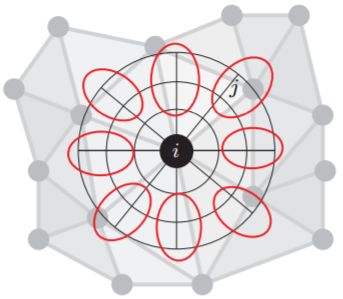
\includegraphics[width=.3\textwidth]{12/22_46_b}
	\caption{Local system of coordinates.}\label{fig:local-coord-weights}	
\end{figure}

So in this system of coordinates we can now express a \emph{localized} \emph{node signal}, that is a function
\begin{equation}
    f: \mathcal{V} \to \mathbb{R}^d
\end{equation}
that associates each node to its $d$ features, and extracting a patch amounts to averaging the function $f$ by these weights, at each point (in the local system of coordinates) where the nodes are localized.

In the same way we can represent also a localized \emph{filter}, i.e. express a function
\begin{equation}
    g: \mathcal{V} \to \mathbb{R}
\end{equation}
that will associate to each point an importance, again multiplied by the proper Gaussian weights. 

Notice that regular convolutional filters enforce locality by being smaller than the image, i.e. giving zero importance to pixels that are outside their range. Here we cannot do the same, so we define the filter on every node, then transform it locally to cover every point in order to enforce locality by means of the same Gaussian weights we used for the node signal.

So then, convolution is defined as the sum of the element-wise products between these weighted, localized node signal and filter:
\begin{equation}
    (f \star g)_i = \vb{f}_i^{\top} \vb{g}, \qquad i = 1, \dots, d
\end{equation}
just like we would convolve a regular convolutional filter and a local patch.

Notice that there is no reason to enforce Gaussian weights specifically, instead of some other weighting mechanism.

\begin{figure}[H]
    \centering
    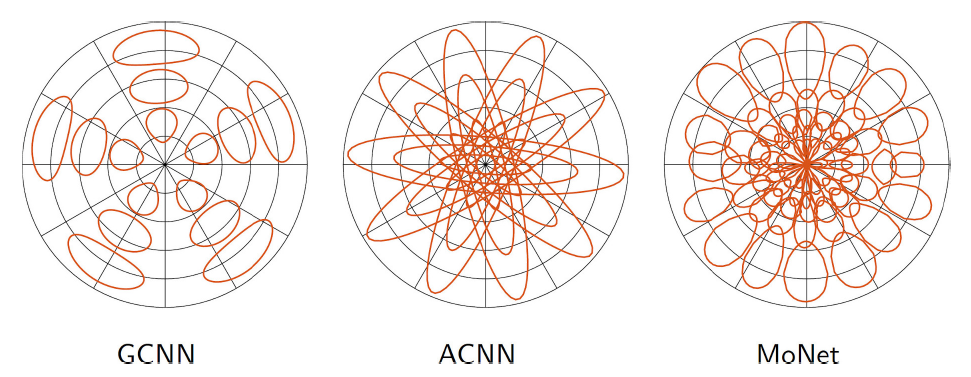
\includegraphics[width=.7\textwidth]{figures/12/monet.png}
    \caption{Different possible weighting mechanism to localize functions in the neighborhood of a point.}
\end{figure}

Many other approaches of this kind are possible, in which one defines convolution spatially as some form of \emph{aggregation} of the node signals from the neighborhood of each node, then \emph{combined} in some way with the representation of the node itself. 

Suppose we have an intermediate hidden representation $\vb{h}_v^{(k-1)}$ for each node $v$ in the graph, at input to the $k$-th convolutional layer. Then the output $\vb{h}_v^{(k)}$ will be
\begin{equation}
    \begin{aligned}
        \vb{a}_{v}^{(k-1)} = \mathrm{AGGREGATE}_k \left( \{ \vb{h}_u^{(k-1)}, ~ u \in \mathcal{N}(v) \} \right) \\
        \vb{h}_{v}^{(k)} = \mathrm{COMBINE}_k \left( \vb{a}_{v}^{(k-1)}, \vb{h}_v^{(k-1)} \right).
    \end{aligned}
\end{equation}
where the $\mathrm{AGGREGATE}_k(\cdot)$ function has the role to enforce locality for this to be a well-behaved convolution-like operator. 